% USE PDFLatex!

\documentclass{popsci}

\usepackage[utf8]{inputenc}
\usepackage[swedish, english]{babel}

\usepackage{fancyhdr}
\usepackage{titling}
\usepackage{color}
\usepackage{colortbl}

\usepackage{lmodern}

\usepackage{graphicx}



\presentationsdag{2018-05-31}

\examensarbete{Improved Sampling for Temporal Anti-Aliasing}
%To create a title in two rows, leave examensarbete blank and fill in examensarbeteTwoRows.
%\examensarbeteTwoRows{Application Specific Instruction-set Processor Using a Parametrizable multi-SIMD}{Synthesizeable Model Supporting Design Space Exploration}

\author{Christian Alexander Oliveros Labrador}
\supervisor {Michael Doggett (LTH)}
\examiner{Flavius Gruian (LTH)}

\title{Improved Sampling for Temporal Anti-Aliasing}


\begin{document}

\theabstract{Real-time Graphic applications, like video games, require solutions for jaggies and pixel flickering in movement problems, aliasing, to render high-quality images. In this thesis, we improved the Temporal Anti-Aliasing technique to provide higher quality images.}


{\noindent Current computer graphics real-time applications strive to provide the highest image quality available at the lowest computational cost possible, they normally need to run at 30 images (frames) per second or more. One of the obstacles to overcome is that normally there is not enough resolution to render everything the best way possible, thus, creating what is commonly referred as jaggies or the blocky look that some rendered images get (formally named Spatial Aliasing); and pixel flickering or jumps in moving objects (Temporal Aliasing).   
	
\begin{figure}[!hbt]
	\centering
	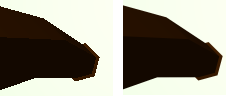
\includegraphics[scale=1.4]{images/pipe_sobel_no_aa.png}
	\caption{Example of Jaggies versus how it should look.}\label{fig:jaggies}
\end{figure}
	
This thesis presents a new approach to Temporal Anti-Aliasing (TAA) that improves on current techniques. TAA works by mitigating the effects of Spatial and Temporal Aliasing using previously rendered frames in the process of rendering the current one. The key benefits that this technique provide are that it solves two types of aliasing problems at the same time; that it is compatible with current rendering pipelines and it provides good results while being lightweight in computational cost. But, applying TAA has two main drawbacks, it generates unnecessary blurriness; and the appearance of trails of objects from previous frames that were moving (ghosting). 

The work of this thesis achieved a reduction in both drawbacks by the use of edge detection, applying the Sobel Operator, by numbering (indexing) models in the scene to differentiate them, and by the use of a new image filter that helps to reduce blurriness without creating more errors. Also, the improvements managed to be at the same level or surpass other Anti-Aliasing solutions, which are common in Real-time Graphic applications. As well, we maintain the low usage of memory and processing time.

The improvement of this Master Thesis were tested using image metrics that represent numerically the quality of an image. This was done in order to corroborate that the improvements were working as intended.
	
}

\end{document}
